% =======================
% Section 6: Notebook
% =======================
\section{Lab}

% ---- Slide 15: Transition to the Notebook Demo ----
\begin{frame}[t]{Lab}

\textbf{Lab: Building an Agentic AI Chatbot}\\[0.3em]
\small From theory to practice: putting the agent loop, tools, and memory to work.\\[0.3em]
\footnotesize \url{https://github.com/awslabs/agentcore-samples/blob/main/01-tutorials/09-AgentCore-E2E/strands-agents/lab-01-create-an-agent.ipynb}

\centering
\vspace{0.5em}
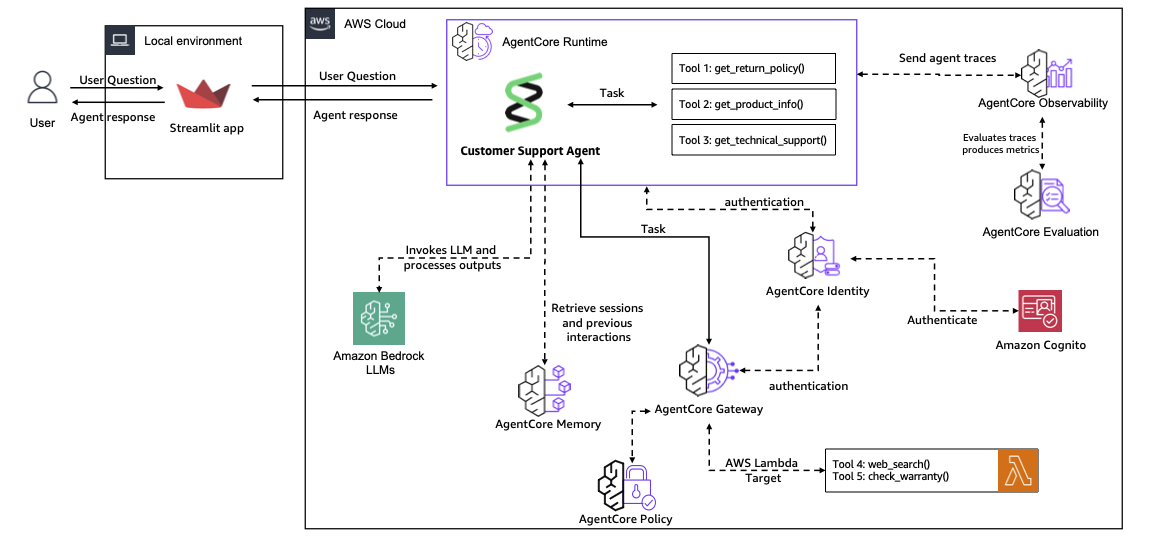
\includegraphics[width=1\textwidth]{images/architecture_lab6_streamlit.png}

% Speaker notes:
% The notebook is intentionally simpler than the full theory stack.
% Not every production concern will be implemented live,
% but students will see the essential agent loop.
\end{frame}
